\documentclass[xcolor={dvipsnames}]{beamer}
\usepackage[utf8]{inputenc}

\usepackage{graphicx}  % For including graphics
\usepackage{subcaption} % For subfigures
\usepackage{caption}   % For customizing captions
\captionsetup[figure]{
  name=,
  singlelinecheck=off,
  labelsep=colon,
  labelfont=bf,
  font=small,
  justification=centering,
}

\usetheme{Madrid}
\usecolortheme{default}
\setbeamertemplate{enumerate items}[default]
\setbeamercolor*{structure}{bg=white,fg=black}

% \setbeamercolor*{palette primary}{use=structure,fg=white,bg=structure.fg}
% \setbeamercolor*{palette secondary}{use=structure,fg=white,bg=structure.fg!75}
% \setbeamercolor*{palette tertiary}{use=structure,fg=white,bg=structure.fg!50!black}
% \setbeamercolor*{palette quaternary}{fg=white,bg=black}

% \setbeamercolor{section in toc}{fg=black,bg=white}
% \setbeamercolor{alerted text}{use=structure,fg=structure.fg!50!black!80!black}
% \setbeamercolor{frametitle}{bg=black,fg=white}

% \setbeamercolor{titlelike}{parent=palette primary,fg=structure.fg!50!black}
% \setbeamercolor{frametitle}{bg=gray!10!white,fg=black}

% \setbeamercolor*{titlelike}{parent=palette primary}

% \setbeamercolor{block title example}{bg=black,fg=white}

% \usepackage{times,url}

% \setbeamertemplate{footline}[frame number]
% \setbeamertemplate{footline}[frame number]{}

\setbeamertemplate{footline}{}

\setbeamertemplate{footline}
% {
%   \leavevmode%
%   \hbox{%
%   \begin{beamercolorbox}[wd=.333333\paperwidth,ht=2.25ex,dp=1ex,center]{author in head/foot}%
%     \usebeamerfont{author in head/foot}\insertsection
%   \end{beamercolorbox}%
%   \begin{beamercolorbox}[wd=.333333\paperwidth,ht=2.25ex,dp=1ex,center]{title in head/foot}%
%     \usebeamerfont{title in head/foot}\insertsubsection
%   \end{beamercolorbox}%
%   \begin{beamercolorbox}[wd=.333333\paperwidth,ht=2.25ex,dp=1ex,right]{date in head/foot}%
%     \usebeamerfont{date in head/foot}\insertshortdate{}\hspace*{2em}
%     \insertframenumber{} / \inserttotalframenumber\hspace*{2ex} 
%   \end{beamercolorbox}}%
%   \vskip0pt%
% }

%------------------------------------------------------------
%This block of code defines the information to appear in the
%Title page
\title[About Beamer] %optional
{Interstellar Interceptors}

\subtitle{Mission design for rendezvous with objects in hyperbolic orbits}

\author[Martínez, Jorge] % (optional)
{
    Jorge Martínez\\
    \vspace{1cm}
    Supervised by:\\
    \vspace{0.5cm}
    Josep M. Trigo-Rodríguez (ICE-CSIC/IEEC)\\
    Eloy Peña-Asensio (Politecnico di Milano)\\
    \vspace{0.5cm}
    \footnotesize{Universidad Internacional de Valencia}
}

\vspace{-0.5cm}
\date{May 22, 2024}

% \logo{\includegraphics[height=1cm]{overleaf-logo}} 

%End of title page configuration block
%------------------------------------------------------------



%------------------------------------------------------------
%The next block of commands puts the table of contents at the 
%beginning of each section and highlights the current section:

\AtBeginSection[]
{
  \begin{frame}
    \frametitle{Table of Contents}
    \tableofcontents[currentsection]
  \end{frame}
}
%------------------------------------------------------------


\begin{document}

%The next statement creates the title page.
\frame{\titlepage}

%---------------------------------------------------------
\begin{frame}
\frametitle{What are interstellar objects?}

\begin{block}{Definition}
    Interstellar objects (ISOs) are asteroids, comets or planetary bodies moving
    through interstellar medium (ISM) without being gravitationally bound to a
    star.
\end{block}

\begin{figure}[h]
    \centering
    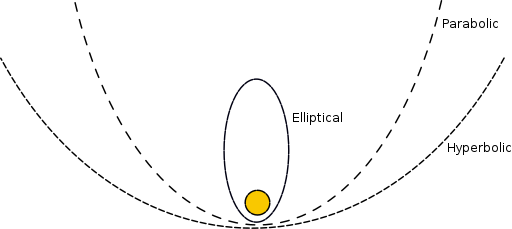
\includegraphics[width=0.75\textwidth]{fig/static/orbits.png}
    \caption{ISOs follow hyperbolic orbits}
    \label{fig:example_figure}
\end{figure}

\end{frame}
%---------------------------------------------------------

%---------------------------------------------------------
\begin{frame}
\frametitle{Why are interstellar objects important?}

They present a unique opportunity to study extraterrestrial bodies that have
traversed vast cosmic distances.\\[0.5cm]

\pause

Their study can unleash information about:\\[0.5cm]

\begin{itemize}
    \item Better understanding the formation of planetary systems
    \item Exploring the origins of life by analyzing their chemical composition
    \item Technological motivation
\end{itemize}

\pause

    \vspace{0.5cm}
    \begin{alertblock}{Motivation of this work}
    \vspace{0.2cm}
    Devise orbits for rendezvous with ISOs to study their physical properties.
    \vspace{0.2cm}
\end{alertblock}

\end{frame}
%---------------------------------------------------------

%---------------------------------------------------------
\begin{frame}
\frametitle{Why are they interesting?}

\begin{figure}
    \centering
    \begin{minipage}{0.45\textwidth}
        \centering
        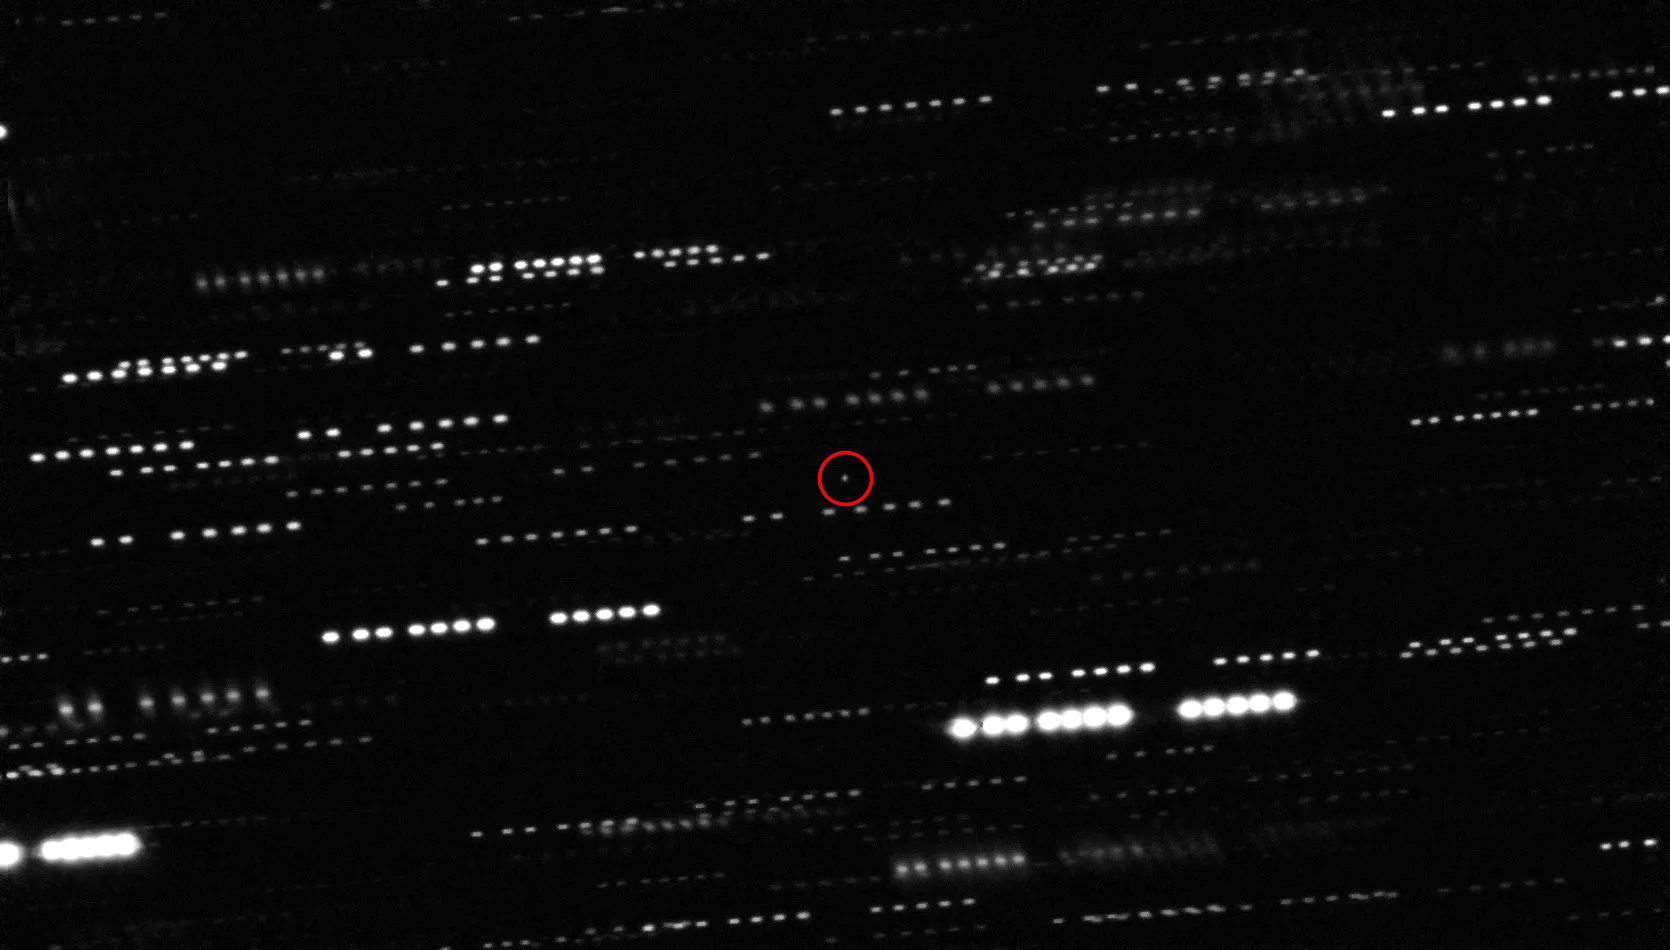
\includegraphics[width=\textwidth]{fig/static/oumuamua/shape.png}
        \caption{1I/'Oumuamua}
        \label{fig:figure1}
    \end{minipage}
    \hfill
    \begin{minipage}{0.45\textwidth}
        \centering
        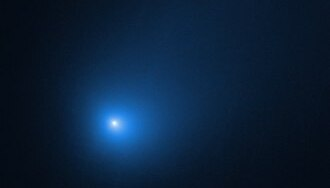
\includegraphics[width=\textwidth]{fig/static/borisov/shape.jpg}
        \caption{2I/Borisov}
        \label{fig:figure2}
    \end{minipage}
\end{figure}


\end{frame}
%---------------------------------------------------------

\section{Second section}

%---------------------------------------------------------
%Highlighting text
\begin{frame}
\frametitle{Sample frame title}

In this slide, some important text will be
\alert{highlighted} because it's important.
Please, don't abuse it.

\begin{block}{Remark}
Sample text
\end{block}

\begin{alertblock}{Important theorem}
Sample text in red box
\end{alertblock}

\begin{examples}
Sample text in green box. The title of the block is ``Examples".
\end{examples}
\end{frame}
%---------------------------------------------------------


%---------------------------------------------------------
%Two columns
\begin{frame}
\frametitle{Two-column slide}

\begin{columns}

\column{0.5\textwidth}
This is a text in first column.
$$E=mc^2$$
\begin{itemize}
\item First item
\item Second item
\end{itemize}

\column{0.5\textwidth}
This text will be in the second column
and on a second tought this is a nice looking
layout in some cases.
\end{columns}
\end{frame}
%---------------------------------------------------------


\end{document}
